\documentclass{article}

\usepackage{geometry}
\geometry{a4paper, margin=1in}

\usepackage{titlesec}
\titleformat{\section}{\large\bfseries}{\thesection.}{1em}{}
\titleformat{\subsection}{\bfseries}{\thesubsection.}{1em}{}

\usepackage{fancyhdr}
\usepackage{graphicx}
\usepackage{booktabs}
\usepackage[hidelinks]{hyperref}\usepackage{xcolor}

\usepackage{tikz}
\usetikzlibrary{shapes,arrows,positioning}


\pagestyle{fancy}
\fancyhf{}
\rhead{\textbf{Apparel Trade in Poland}}
\lhead{\today}
\rfoot{Page \thepage}

\begin{document}

\begin{titlepage}
    \centering
    \vspace*{4cm}
    {\Huge\bfseries Understanding the Apparel Market: \\ Trading in Poland \par}
    \vspace{2cm}
    {\large A Comprehensive Overview \par}
    \vfill
    \vspace{2cm}
    {\large \today\par}
\end{titlepage}

\newpage
\tableofcontents
\newpage    

\section{Introduction}
Poland's apparel market offers a wealth of opportunities for businesses. It's a vibrant and diverse landscape where tradition meets modernity. Success in this realm requires a deep understanding of product categories, effective sales strategies, and an awareness of the myriad external factors that influence sales. This document aims to provide an in-depth understanding of the various nuances of the Polish apparel market.

\section{Business Model}

The company operates based on a direct sourcing and distribution model, which can be described in the following steps:

\begin{enumerate}
    \item \textbf{Product Design and Sourcing:} 
    The company either sources pre-designed products or creates custom designs tailored to specific needs. For custom designs, the company conceptualizes the design and then collaborates with manufacturing entities in China to bring these designs to life.

    \item \textbf{Production:} 
    With the designs in hand, the products are then manufactured in specialized factories located in China. These factories are equipped to produce protective gear that meets both the design specifications and any required safety standards.

    \item \textbf{Distribution and Sales:} 
    Once the products are manufactured and ready for the market, the company takes on the role of distributor. They sell these products to:
    \begin{itemize}
        \item DIY shops, like Leroy Merlin.
        \item Wholesalers who specialize in the distribution of protective gear.
    \end{itemize}

    \item \textbf{End Consumers:} 
    The DIY shops and wholesalers, in turn, sell these products to the end consumers. The primary target for these products are companies that require protective gear for their industrial operations. However, there is also a retail segment where individual consumers can purchase these products for personal use.
\end{enumerate}

Here is visualization of above described business model:

\begin{center}
    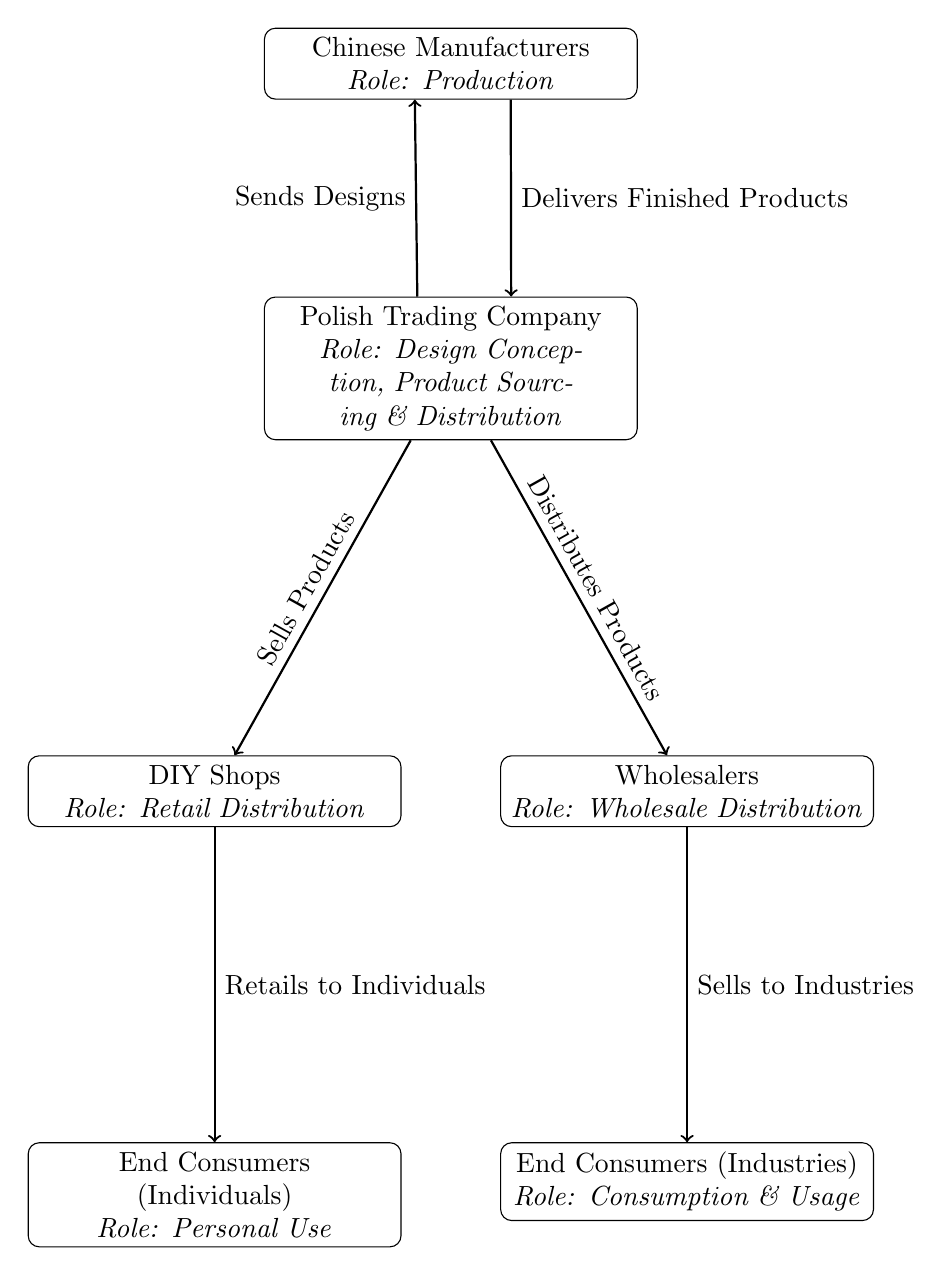
\begin{tikzpicture}[node distance=2.5cm, auto]
        % Nodes
        \node[draw, rectangle, rounded corners, text width=4.5cm, align=center] (company) {Polish Trading Company \\ \textit{Role: Design Conception, Product Sourcing \& Distribution}};
        \node[draw, rectangle, rounded corners, text width=4.5cm, align=center, above=of company] (manufacturers) {Chinese Manufacturers \\ \textit{Role: Production}};
        \node[draw, rectangle, rounded corners, text width=4.5cm, align=center, below=of company, yshift=-1.5cm, xshift=-3cm] (shops) {DIY Shops \\ \textit{Role: Retail Distribution}};
        \node[draw, rectangle, rounded corners, text width=4.5cm, align=center, below=of company, yshift=-1.5cm, xshift=3cm] (wholesalers) {Wholesalers \\ \textit{Role: Wholesale Distribution}};
        \node[draw, rectangle, rounded corners, text width=4.5cm, align=center, below=of shops, yshift=-1.5cm] (individuals) {End Consumers (Individuals) \\ \textit{Role: Personal Use}};
        \node[draw, rectangle, rounded corners, text width=4.5cm, align=center, below=of wholesalers, yshift=-1.5cm] (consumers) {End Consumers (Industries) \\ \textit{Role: Consumption \& Usage}};
    
        % Arrows
        \draw[->, thick] (company.115) -- (manufacturers.945) node[midway, left, align=center] {Sends Designs};
        \draw[->, thick] (manufacturers.689) -- (company.50) node[midway, right, align=center] {Delivers Finished Products};
        \draw[->, thick] (company) -- (shops) node[midway, above, sloped, align=center] {Sells Products};
        \draw[->, thick] (company) -- (wholesalers) node[midway, above, sloped, align=center] {Distributes Products};
        \draw[->, thick] (shops) -- (individuals) node[midway, right, align=center] {Retails to Individuals};
        \draw[->, thick] (wholesalers) -- (consumers) node[midway, right, align=center] {Sells to Industries};
    \end{tikzpicture}
    \end{center}

\section{Key Considerations}
\begin{itemize}
    \item \textbf{Sales Planning:} Preparation is crucial. When approaching large retail chains, businesses must anticipate their needs. This might mean bolstering their workforce in advance of significant sales events, ensuring that customer demands are met efficiently.
    \item \textbf{Market Trends:} Poland boasts a unique blend of local and international fashion preferences. Recognizing and catering to this balance can set a business apart, allowing them to connect more effectively with their target audience.
\end{itemize}

\section{Categorizing Apparel}
Understanding the different categories of apparel can help businesses strategize effectively.
\subsection{By Demand}
\begin{itemize}
    \item \textbf{Seasonal Apparel:} Products like winter jackets and summer sandals are influenced by the changing seasons. Anticipating these shifts can lead to optimized sales.
    \item \textbf{Evergreen Apparel:} Certain staples, such as t-shirts and jeans, are consistently in demand, making them essential inventory items.
\end{itemize}
\subsection{By Function}
\begin{itemize}
    \item \textbf{Upper Body Wear:} This category, including jackets and shirts, is vast and caters to both daily wear and specific occasions.
    \item \textbf{Headgear:} From fashionable hats to protective helmets, this category serves both function and style.
    \item \textbf{Leg Wear and Protection:} Beyond daily wear like trousers, this category also includes specialty items like protective gear.
\end{itemize}

\section{Effective Sales Approaches}
\begin{itemize}
    \item \textbf{Bundling Products:} Offering products as sets, such as a jacket with matching gloves, can enhance sales appeal. Such bundles can offer customers better value and enhance their shopping experience.
    \item \textbf{Identifying Target Audiences:} A clear understanding of the target market, whether it's the general public or niche groups, can lead to more tailored and effective sales strategies.
\end{itemize}

\section{Influences on Sales}
Numerous external factors can sway consumer purchasing decisions.
\begin{itemize}
    \item \textbf{Economic Climate:} The broader economic health can influence consumer spending habits, with downturns leading to more conservative buying behavior.
    \item \textbf{Fashion Shifts:} The ever-evolving world of fashion can drastically impact the popularity of certain apparel items.
    \item \textbf{E-commerce Trends:} As the digital age progresses, online shopping continues to reshape traditional buying patterns.
    \item \textbf{Regulatory Environment:} Changes in government regulations, trade policies, or import/export tariffs can affect both sales and manufacturing practices.
    \item \textbf{Sustainability Concerns:} With increasing global emphasis on eco-friendly practices, sustainable and ethically-produced apparel is gaining traction.
\end{itemize}

\section{Understanding Sales Data}
Data-driven insights can greatly benefit businesses.
\begin{itemize}
    \item \textbf{Data Source:} The sales data under discussion originates from a specific trading company, providing a snapshot of its market performance.
    \item \textbf{Leveraging Data:} Analyzing this data can offer invaluable insights into consumer behavior, future trends, and areas of improvement. This allows businesses to refine their strategies and anticipate market shifts.
\end{itemize}

\section{Conclusion}
The apparel market in Poland is both challenging and rewarding. For businesses to thrive, they must stay informed, adaptable, and proactive. With the right blend of market understanding, sales strategy, and responsiveness to external influences, success is not just possible—it's probable.





    

\end{document}